%\section{Facility Location}

In this chapter, we will present the main results of the Facility Location Problem in more detail. To better understand the problem, we will start with some useful definitions from the relevant field of Social Choice. Then we will formally define the setting and the basic concepts of \emph{Algorithmic Mechanism Design}.

\section{Social Choice and Single Peaked Preferences}

Social choice theory is the study of collective decision processes and procedures. How can a group of individuals choose a winning outcome (e.g., policy, electoral candidate) from a given set of options? In the most general setting there is a set $N$ of $n$ agents and a set $\A$ of alternatives. Each agent has a private order of the alternatives $\succ_i$ over the alternatives in $\A$. Let $L$ be the set of all linear orders of $\A$. A \emph{social choice function} $f:L^n \rightarrow \A$ maps the agents' preferences to a single alternative. A social choice function must satisfy the following properties:
\begin{definition}[Unanimous]
A social choice function $f$ is unanimous if, when all player prefer a certain outcome more than anything else, then that outcome must be the alternative chosen by the mechanism. That is, if $\exists a \in\A$ such that $\forall b\in\A$ and $i \in  N$, $a \succ_i b$ then $f(\succ_1,...,\succ_n) =a$.
\end{definition}
\begin{definition}[Onto]
 A social choice function $f$ is onto if any alternative can be reached given the appropriate preference profiles That is, $\forall a \in\A$, $\exists \x\in L^n$ such that $f(\x) = a$.
\end{definition}
\begin{definition}[Pareto Optimal]
 A social choice function $f$ is Pareto optimal if no other alternative is more preferred by every agent than the alternative chosen by the mechanism. That is, if $f(\x)=a$ for a $\x\in L^n$, then $\nexists b\in\A$ such that $b\succ_i$, $\forall i \in N$.
\end{definition}
\begin{definition}[Strategyproof]
A social choice function $f$ is strategyproof if no agent can change the outcome to a more preferable by misreporting her preferences. That is, for all preference profiles $\succ_1,...,\succ_n$ and any agent $i$, and any alternative preference $\succ_i'$: $f(\succ_1,...,\succ_i,...,\succ_n) \succ_i f(\succ_1,...,\succ_i',...,\succ_n)$.
\end{definition}

Our goal is to find the best possible outcome given the agents' preferences. The first three properties ensure that the selected outcome is efficient, namely desirable for all the agents. The agents, on the other hand, are selfish and strategic, aiming to maximize their utility. This is why, if we want the social function to be fair, the fourth property is crucial.

An other important property of social choice function is \emph{anonymity}, namely that the selection is based on the preference profiles only and not on the agent reporting it. This implies that all agents count the same in decision making.
\begin{definition}[Anonymous]
A social choice $f$ is anonymous if for all permutations $\pi$ and all profiles $(\succ_1,...,\succ_n)\in L^n$: $f(\succ_1,...,\succ_n) =f(\succ_{\pi(1)},...,\succ_{\pi(n)})$ 
\end{definition}

There are social choice functions that do not satisfy anonymity. For example, a \emph{dictatorial} social choice function that always selects the most preferred alternative for a particular agent, ignoring the preference profiles of the rest of the agents. We will call this agent a dictator. A dictatorial social choice function is strategyproof and Pareto optimal, but not fair because not all agents count the same.


\begin{definition}[Dictator]
An agent $i$ is a dictator in a social choice function $f$ if for all $\succ_1,...,\succ_n\in L$: $f(\succ_1,...,\succ_n)=a$ where $a\succ_i b, \forall b\in \A$ with $b\ne a$.
\end{definition}



A simple and intuitive example of a social choice function is the majority vote. If there are only two alternatives then the majority is strategyproof. If there are $3$ or more alternatives, however, the majority is not strategyproof. An agent may change her preference profile to prevent her least liked option from being selected. Unfortunately, there is an impossibility result that states we cannot do anything better than a dictatorship when there are more that 3 alternatives. 



\begin{theorem}[Gibbard \cite{Gibbard1973} - Satterthwaite \cite{Satterthwaite1975}]
Let $f$ be an incentive compatible
social choice function onto $\A$, where $\A \ge 3$, then $f$ is a dictatorship.
\end{theorem} 

One way to overcome the impossibility result of the previous theorem is to introduce payments into the model. There are many strategyproof mechanisms with money. The idea is that if an agent misreports in an attempt to benefit, the extra payment from the mechanism will be more than the actual decrease in the cost. However, as we mentioned before, we are interested in applications where payments are not an option. So, in order to overcome the impossibility result without money, we are going to restrict the domain of possible preference profiles to single-peaked preferences. Preferences are said to be single-peaked if the alternatives can be represented as points on a line, and each agent has a unique most preferred point (``"peak" preference) and points that are further from her peak are preferred less. It is natural to assume that the agents have single-peaked preferences for many problems. For example, in the Facility Location setting, where the government wants to place public facilities, any agent would prefer the facility closest to her ideal location since any other facility will only increase the transportation cost.


\begin{definition}[Single-Peaked Preferences]
Preferences are said to be single-peaked if the alternatives can be represented as points on a line, and there exists an alternative $a \in \A$ (the peak) such that if $x<y<a \implies y \succ x$ and if  $a<x<y \implies x\succ y$. 
\end{definition}

Moulin \cite{Moulin1980} showed that if all the agents have single-peaked preferences, there exists a strategy-proof mechanism that only depends on the peak of each agent.


\begin{theorem}
Assuming single peakedness, a rule $f$ is strategyproof, onto and anonymous if and only if there exists $a_1,a_2,...,a_n\in [0,1]$ such that for all peaks $(x_1,...,x_n)\in \mathbb{R}$.
\end{theorem}




\section{Preliminaries for Facility Location Games}

By the definition of single-peaked preferences we can see that a profile is single-peaked if for any two points on the same side of the peak the agent always prefers the one which is closer to her peak. But there is no way to now by ``how much" agent $i$ prefers alternative $x$ over $y$. From now on, we are going to assume that the agents rank the all the alternative locations based on the distance from their peak.


\begin{definition}[Facility Location]
Let $N= \{1,..,n\}$ be a set of agents. The agents are located in a metric space $(X,d)$, where $d:X \times X \rightarrow  \mathbb R_{\ge 0} $ is the distance function. The function $d$ is a metric on $X$ satisfying $d(x,x)=0$ for all $x\in X$, $d(x,y)=d(y,x)$ for all $x,y\in X$ (\emph{symmetry}) and, $d(x,z)\le d(x,y)+d(x,z)$ for all $x,y,z\in X$ (\emph{triangle inequality}). Each agent $i\in N$ has a private location $x_i \in X$. We refer to the tuple $\x=(x_1,...x_n)$ as the \emph{location profile} or \emph{instance}.
\end{definition}


For a location profile $\x$ and an agent $i$, let $\x_{-i}$ denote the tuple $\x$ without the coordinate $x_i$. Similarly, for a non-empty set $S$ of indices, let $\x_S=(x_i)_{i\in S}$ be the locations of agents in $S$ and $\x_{-S}=(x_i)_{i\notin S}$ the tuple $\x$ without the location of agents in $S$.  

Each agent reports her ideal location to the mechanism $M$. A \emph{deterministic mechanism} $M$ for $k$-Facility Location maps an instance $\x$  to a $k$-tuple $\vec{c}=(c_1,...,c_k)\in X^k$. We let $M(\x)$ denote the outcome of $M$ in instance $\x$. Similarly, a \emph{randomized mechanism} $M$ maps an instance $\x$ to a probability distribution over $k$-tuples $(c_1,...,c_k)\in X^k$.

For a location profile $\x$ and a mechanism $M$, we define the \emph{connection cost} of agent $i$ as the minimum distance of her private location to the closest facility, $cost(x_i,M(\x)) = min_{1\le j \le k} \{d(x_i,c_j) \}$. The \emph{social cost} of a mechanism $M$ is the total distance of the agents' locations to the nearest facility, $cost(\x,M(\x)) = \sum_{i=1}^n d(x_i,M(\x))$. 
%The \emph{maximum cost} of $M$ is the maximum distance of an agent to her closest location, $MC(\x,M(\x)) =  max_{i\in N } \{ d(x_i,M(\x))\}$

Since each agent is strategic, it is easy to see that the goal of each agent is different from the mechanism's. The mechanism's objective is to minimize the social cost, but each strategic agent seeks to minimize its connection cost. This divergence between the two goals motivates an agent to manipulate the mechanism by reporting a false location to achieve a better connection cost. This is why strategyproofness is a crucial property that any mechanism should satisfy.

\begin{definition}[Strategyproof]
A mechanism is strategyproof if for all location profiles $\x$, any agent $i$, and all locations $y$: 
\[cost(x_i,M(x)) < cost(x_i, M(x_{-i},y))\]
\end{definition}

A mechanism can also be \emph{group strategyproof} if for any coalition misreporting their location simultaneously, at least one does not benefit. Formally: 
 
\begin{definition}[Group Strategyproof]
A mechanism is strategyproof if for location profiles $\x$, all coalitions $S \subset N$ and all location profiles $\xx = (\x_{-S},x_S')$, there exists an agent $i\in S$ such that
\[ cost(x_i,M(\x)) \le cost(x_i,M(\xx))\]
\end{definition}

\begin{definition}[Image Set]\label{imageSet}
For any mechanism $M$, the \emph{image set} of agent $i$ with respect to a location profile $\x_{-i}$ is the set of all the possible facility locations the agent can obtain by varying her reported location. Formally:
\[ I_i(\x_{-i}) = \{a \in  X: \exists \;y \in X \; with \; M(\x_{-i},y)\}\]
\end{definition}

We can see the image set as the power an agent has on the mechanism. Any strategyproof mechanism $M$ always outputs some location in $I_i(\x_{-i})$ that is closest to the reported location as shown in the following lemma.

\begin{lemma}\label{imageSetLemma}
Let $M$ be a strategyproof mechanism for the $k$-Facility game. For every location profile $\x \in X^n$ and any agent $i\in N$ we have:
\[ cost(y,M(\x_{-i},y)) = \inf_{a\in I_i(\x_{-i})} \{d(a,y)\}\]
\end{lemma}

\begin{proof}
For the location profile $\xx=(\x_{-i},y)$ let $a\in M(\xx)$. Assume for contradiction that exists $a^*\in I_i(\x_{-i})$ such that $d(a^*,y) < d(a,y)$. By the definition of the image set there exists a $y^*$ such that $a^* \in M(\x_{-i},y^*)$. Then, if agent $i$ is located at y she can benefit by misreporting to $y^*$ lowering her connection cost from $cost(y, M(\x_{-i},y))$ to $d(a^*,y)$. This contradicts the assumption that $M$ is strategyproof
\end{proof}

We can extend the previous definition of image set from a single agent to a group of agents. For a given mechanism $M$ we define the image set of agents in a subset $S$ with respect to a location profile $\x_{-S}$ as the set of all possible facility locations they can obtain by varying their reported location:

\[ I_S(\x_{-S}) = \{a \in X: \exists\;\vec{y} \in X^{|S|} \; with \; M(\x_{-S},\vec{y})\}\]

We can also extend the previous lemma to hold for partial group strategyproof mechanisms, when all agents in the coalition report the same location.
\begin{lemma}
Let $M$ be a strategyproof mechanism for the $k$-Facility Location game. For every location profile $\x \in X^n$, any non-empty set of agents $S\subset N$, $\vec{y}$ and $\vec{y}=(y,...,y)$ we have:
\[ cost(y,M(\x_{-S},\vec{y})) = \inf_{a\in I_S(\x_{-S})} \{d(a,y)\}\]
\end{lemma}


%\section{Facility Location}

%introo  single peak preference and distance function 

\section{Facility Location on the Line}

In this section, we are going to focus on \emph{Facility Location} on the real line. Let $N=\{1,...,n\}$ be the set of agents. Each agent has a private ideal location $x_i\in \mathbb{R}$. We can assume without loss of generality that the locations in the location profile $\x = (x_1, ..., x_n)$ are ordered ($x_1\le x_2\le...\le x_n$), since we focus on anonymous mechanisms. Given an instance $\x$ the most important locations are the leftmost and the rightmost because they delimit the instance. We denote the leftmost location as $lt(\vec{x})=min_{i\in N}\{x_i\}$ and the rightmost location as $rt(\vec{x})=max_{i\in N}\{x_i\}$. The distance function between any two locations is simply the length of the interval, $d(x,y) = |x-y|$. 
%{+??+}


%----------------------------------------------------------------------------
%One facility on the line
\subsection{Locating one facility}

We start with the simplest setting. Given an instance $\x$ we want to place one facility that achieves the best possible social cost in a strategyproof way. 

\begin{theorem}
The mechanism that selects the median location of the reported instance is strategyproof and optimal for the social cost objective.
\end{theorem}

\begin{proof}
We first show that the median location, $med(\vec{x})$, is the optimal solution. If $n$ is odd the median location is $x_{(n+1)/2}$, if $n$ is even any location in the interval $[x_{n/2},x_{n/2+1}]$ is optimal without lost of generality we consider $x_{n/2}$ to be the selected location. Suppose the facility is placed at a location to the left of the median location, let that location be $x$. Then, at least half of the agents' connection cost has increased by $d(x,med(\vec{x}))$, and at most half of the agents' connection cost has decreased by $d(x,med(\vec{x}))$. This makes the social cost of $x$ higher than the optimal. The same holds for any location selected to the right of the median.

We now show that the mechanism is strategyproof. The agent located at $med(\vec{x})$ has no initiative to misreport her location, since her connection cost is zero. Suppose an agent $i$ located at $x_i$ misreports to $x_i'$. Without loss of generality we can assume that $x_i<med(\vec{x})$. If $x_i'<med(\vec{x})$ then the output of the mechanism does not change. If $x_i'>med(\vec{x})$ the median location moves to the right leading to an increase in her cost.
\end{proof}



%------------------------------------------------------------
%Two Facilities on the Line

\subsection{Locating two facilities}
This section extends the previous setting from locating one facility on the real line to locating two. Now a mechanism returns a 2-tuple $\vec{c}=(c_1,c_2)$ with the location of the facilities; we can assume that $c_1 \le c_2$. Each agent connects to the nearest facility with connection cost equal to $cost(x,\vec{c})=min\{ d(x,c_1), d(x,c_2)\}$. 


Let us focus on the optimization problem of locating the two facilities without considering the strategic agents' motives. Let $\vec{x}$ a location profile, and $c_1$,$c_2$ the optimal facility locations.  We can split the agents into two (non-empty) groups based on which facility they prefer. The agents that prefer $c_1$ belong to the "left" set $L(\vec{x})$, and the rest belong to the "right" set $R(\vec{x})$. Using the same argument as in the previous setting for one facility on the line, given the sets $L(\vec{x})$ and $R(\vec{x})$, the optimal locations $c_1$ and $c_2$ are the median of each set. So, for an arbitrary location profile $\vec{x}$, we can compute the optimal solution by selecting the locations that minimize the social cost over the (n-1) choices for $L(\vec{x})$ and $R(\vec{x})$.

%%%????????????????????????
Unfortunately, the mechanism that selects the optimal solution is not strategyproof. The reason is that the sets in the optimal solution are susceptible to minor changes, and the agents can benefit from that. In order to design a strategyproof mechanism we need to extract $L(\vec{x})$ and $R(\vec{x})$ in a strategyproof way. Since both sets are non-empty we are sure that the leftmost agent belongs to $L(\vec{x})$ and the rightmost agent to $R(\vec{x})$. So the mechanism that places the facilities to the leftmost and the rightmost agent is strategyproof and achieves $(n-2)$-approximation ratio. As we will see bellow this is the only deterministic anonymous strategyproof mechanism with bounded approximation for the $2$-Facility Location game. 

\begin{theorem}
The \textsc{Two Extremes} mechanism that places the facilities at the leftmost $lt(\vec{x})$ and the rightmost $rt(\vec{x})$ is a $(n-2)$-strategyproof mechanism for social cost.
\end{theorem}
\begin{proof}
To show the approximation ratio consider the location profile with $n$ agents, where one agent is located at 0, $n-2$ agents are located at $\epsilon>0$ (arbitrarily close to 0), and one agent at 1. The optimal solution places one facility at $\epsilon$ and the other at $1$. The social cost of the optimal solution is $SC^* = \epsilon$. The social cost of the solution outputted by the mechanism is $(n-2)\epsilon = (n-2) SC^*$, since $(n-2)$ agents have connection cost equal to $\epsilon$.

We now show that the mechanism is also strategyproof. Let $\vec{x}$ be a location profile. Any agent reporting a location in the interval $[lt(\vec{x}),rt(\vec{x})]$ cannot change the output of the mechanism. However, if an agent reports a location $x' \in (-\infty,lt(\vec{x})) \cup (rt(\vec{x}),\infty)$ will move the facility further away from her ideal location. So, no agent can benefit by misreporting her location
\end{proof}



%-------------------------------------------------------------------------

In the paper \cite{Procaccia2013} Procaccia and Tennenholtz proved that any deterministic strategy proof mechmanism for 2-Facility Location game has approximation ratio of at least $1.5$. This result was later improved to $2$ \cite{Lu2009}, and then to $(n-1)/2$ \cite{Lu2010} . Fotakis and Tzamos \cite{Fotakis2014} proved a tight lower bound of $n-2$. From the latest result we conclude that the \textsc{Two Extremes} mechanism is the only deterministic, anonymous, strategy-proof mechanism with a bounded approximation ratio.  


The takeaway from the previous section is that we cannot improve the linear approximation ratio for any deterministic strategyproof mechanism. So, the next question is if we can achieve better results with randomized mechanisms. Fortunately, the answer is yes. The \emph{Proportional Mechanism} \cite{Lu2010} is strategyproof and achieves a constant approximation ratio. The idea for this mechanism is very simple and intuitive. Place the first facility uniformly at random among all the reported locations and the second with a probability proportional to its distance from the first. However, is not that simple to prove that the mechanism is indeed strategyproof with constant approximation ratio.

\begin{definition}[Proportional Mechanism]

Given a location profile $\vec{x}=(x_1,...x_n)$, the location of the two facilities are decided by the following random process:
\begin{itemize}
    \item\textbf{Round 1:} Choose agent $i$ uniformly at random from $N$. The first facility $c_1$ is placed at $x_i$

    \item\textbf{Round 2:} Let $d_j = d(c_1,x_j)$ be the distance from agent $j$ to the first facility. Choose agent $j$ with probability $\frac{d_j}{\sum_{k\in N}d_k}$. The second facility is placed at $x_j$.

\end{itemize}
\end{definition}




\begin{theorem}
The proportional mechanism for the two-Facility Location game is strategyproof.
\end{theorem}
\begin{proof}
Let $cost_k(x_i,M(\x))$ denote the expected cost of agent $i$ when the mechanism places the first facility facility on $x_k$. The agent that has a facility at her location experiences after the first round zero cost, so $cost_k(x_k,M(\x))=0$. Since the first facility is selected uniformly at random, we have that for any agent $i$ her total cost is:
\[ cost(x_i,M(\x)) = \frac{1}{n}\sum_{k=1}^{n} cost_k(x_i,M(\x)) = \frac{1}{n}\sum_{k\ne i} cost_k(x_i,M(\x)) \]



Let $\xx=(\x_{i},x_i')$ be the location profile after the deviation of agent $i$. We need to show that she cannot decrease her cost by misreporting her location. We need to show that for all $k\ne i$:

\[ cost(x_i,M(x)) < cost(x_i, M(\xx))\]

Fix the first facility on $x_k$. The expected cost of agent $i$ to the second facility, conditional on the first facility is at $x_k$, is:
\[ cost(c_2,x_i) = \sum_{j=1}^{n} { Pr[c_2=x_j]\cdot d(x_i,x_j)} = \sum_{j=1}^{n} { \frac{d_j}{\sum_{k=1 }^{n}d_k} d(x_i,x_j)}  = \frac{ \sum_{j=1}^{n}d_j \cdot d(x_i,x_j)}{\sum_{j=1}^{n}d_j} \]

Then we have that the cost of agent $i$ is the minimum between the distance to $x_k$ and the expected distance to the second facility:

\begin{align*}
   cost_k(x_i,M(\x)) &= \min\bigg\{d_i, \frac{ \sum_{j=1}^{n}d_j \cdot d(x_i,x_j)}{\sum_{j=1}^{n}d_j}  \bigg\}\\
   &= \frac{\sum_{j=1}^{n}d_j \min\{d_i,d(x_i,x_j)\}}{\sum_{j=1 }^{n}d_j}\\
   &= \frac{\sum_{j\neq i}d_j \min\{d_i,d(x_i,x_j)\}}{\sum_{j=1 }^{n}d_j}
\end{align*}

Let $d_i'=d(c_1,x_i')$. The cost of agent $i$ if she misreports is:
\[ cost_k(x_i,M(\xx)) =\frac{\sum_{j\neq i}d_j \min\{d_i,d(x_i,x_j)\}}{\sum_{j=1 }^{n}d_j + (d_i'-d_i)} + \frac{d_i' \min\{d_i,d(x_i,x_i')\}}{\sum_{j=1 }^{n}d_j + (d_i'-d_i)} \]

We can get the following relation between $cost_k(x_i,M(\x))$ and $cost_k(x_i,M(\xx))$:

\begin{equation}\label{compCost}
cost_k(x_i,M(\xx)) =\frac{ cost_k(x_i,M(\x)) \sum_{j=1}^{n}d_j }{\sum_{j=1 }^{n}d_j + (d_i'-d_i)} + \frac{d_i' \min\{d_i,d(x_i,x_i')\}}{\sum_{j=1 }^{n}d_j + (d_i'-d_i)}    
\end{equation}


We need to distinguish two cases:
\begin{enumerate}[(i)]
    \item $d_i' \le d_i$: we have that $cost_k(x_i,M(\x)) < cost_k(x_i,M(\xx))$ because $\frac{\sum_{j=1}^{n}d_j }{\sum_{j=1 }^{n}d_j + (d_i'-d_i) }>1$ and the second term in the previous equality is non-negative.
    \item $d_i' > d_i$: This case is not that simple. If we subtract $cost_k(x_i,M(\x))$ from (\ref{compCost}), we have:
\[ cost_k(x_i,M(\xx)) - cost_k(x_i,M(\x)) =\frac{ -(d_i'-d_i)cost_k(x_i,M(\x))  }{\sum_{j=1 }^{n}d_j + (d_i'-d_i)} + \frac{d_i' \min\{d_i,d(x_i,x_i')\}}{\sum_{j=1 }^{n}d_j + (d_i'-d_i)}\]

So it suffice to show that:
\begin{equation}\label{s}
   d_i' \min\{d_i,d(x_i,x_i')\}-(d_i'-d_i)cost_k(x_i,M(\x)) \ge 0 
\end{equation}

We need to show that (\ref{s}) holds for both cases:
    \begin{enumerate}
        \item If $\min\{d_i,d(x_i,x_i')\} = d_i$. We have that $d_i \ge cost(x_i,M(\x))$ because agent $i$ always selects the facility closest to her location which cannot be further than the facility placed ad $x_k$. We also have $d_i' \ge d_i' - d_i$. By multiplying the previous inequalities we have that (\ref{s}) holds.
        \item If $\min\{d_i,d(x_i,x_i')\} = d(x_i,x_i')$. We have that $d_i'=d_i \ge cost(x_i,M(\x))$. From triangle inequality we have $d(x_i,x_i') \ge d_i'-d_i$. Again by multiplying the previous inequalities we get that (\ref{s}) holds.
    \end{enumerate}
\end{enumerate}

\end{proof}

It is very interesting that an agent cannot gain even if she knows where the first facility is placed after the first round.

\begin{theorem}
The approximation ratio of the Proportional mechanism for the two Facility Location game is 4 for any metric space.
\end{theorem}

The proportional mechanism is the best know randomized strategyproof mechanism for 2-Facility Location game. The previous know result \cite{Lu2009} has an approximation ratio of $n/2$. A a constant upper bound is a great improvement to the previous liner bound, but there is still a big gap between the upper bound and the only know lower bound for randomized mechanisms, which is $1.045$\cite{Lu2009}. 




\subsection{Locating more than two facilities}

As we previously saw the problem becomes significantly more difficult when we want to locate two facilities instead of one. For the 2-Facility Location games we saw that \textsc{Two Extremes} is the only deterministic and it has a linear approximation ration. Therefore, we cannot expect any better results for $k$-facility location games, when $k\ge3$. In fact we have a very negative result: there is no deterministic anonymous strategyproof mechanism with bounded approximation for $k\ge3$ \cite{Fotakis2014}. This holds even for $n=k+1$ agents. We are going to focus on the intuition behind the proof and present a sketch-proof.  We will refer to deterministic, anonymous, and strategyproof mechanisms with a bounded approximation ratio (in terms of $n$ and $k$) as \emph{nice mechanisms}.



The proof heavily relies at \emph{well-separated instances}, namely instances with $k-1$ isolated agents and two nearby agents. Let $\x = (x_1|x_2|...|x_k, x_{k+1})$ be a well separated instance. The optimal solution is to serve all the isolated agents by a different facility and the two nearby by from the remaining facility. First, we are going to show some properties of nice mechanisms. 

%Given a nice mechanism $M$ with an approximation ration $\rho$ ----- an $a$-approximation mechanism $M$  includes a pair of nearby agents at distance to each other less than $1/a$ times the distance between any other pair of consecutive agents. 


\begin{proposition}
Let $M$ be a nice mechanism for $k$-Facility Location on the line. For any $(k+1)$-location instance $\x$, $M_1(\x) \le x_2$ and $M_k(\x)\ge x_k$
\end{proposition}


\begin{proposition}
Let $M$ be a nice mechanism for $k$-Facility Location. For any $\x=(x_1|x_2|...|x_k,x_{k+1})$ well separated instance, $M_k(\x) \in [x_k,x_{k+1}]$
\end{proposition}

The following propositions show that in well-separated instances if a mechanism places a facility on the left of the nearby agents and we ``push" both agents to the right, while keeping the instance well-separated, the rightmost facility remains on the same agent. Similarly, if a mechanism places a facility on the right of the nearby agents and we ``push" both agents to the left then the rightmost facility remains on the same agent. 

\begin{proposition}
Let $M$ be a nice mechanism for $k$-Facility Location and let  $\x = (x_1|x_2|...|x_k,x_{k+1})$ be a well separated instance such that $M_k(\x) = x_k$. Then for every $\xx = (\x_{-\{k,k+1\}},x_k',x_{k+1}')$ well separated instance with $x_k \ge x_k'$ it holds $M_k(\xx) = x_k'$
\end{proposition}


\begin{proposition} \label{left}
Let $M$ be a nice mechanism for $k$-Facility Location and let  $\x = (x_1|x_2|...|x_k,x_{k+1})$ be a well separated instance such that $M_k(\x) = x_{k+1}$. Then for every $\xx = (\x_{-\{k,k+1\}},x_k',x_{k+1}')$ well separated instance with $x_{k+1} \le x_{k+1}'$ it holds $M_k(\xx) = x_{k+1}'$
\end{proposition}

Using the previous propositions we can show that any anonymous nice mechanism for $k$-facility location on $(k+1)$-agent instances always allocates facilities to the leftmost and to the rightmost agent.

\begin{lemma}\label{leftRight}
Let $M$ be a nice mechanism for $k$-Facility Location with $k\ge2$ and $n=k+1$. Then for all instances $\x=(x_1,...,x_{k+1})$ with $x_1\le...\le x_{k+1}$, $M_1(\x) = x_1$ and $M_k(\x)=x_{k+1}$.
\end{lemma}

We can now show that there is no nice mechanism for $k$-Facility Location when $k\ge3$.

\begin{theorem}
For every $k\ge3$, any deterministic strategyproof mechanism for $k$-Facility Location with $n\ge k+1$ agents on the line has an unbounded approximation ratio. 
\end{theorem}
The previous propositions and the lemma describe how any nice mechanism should ``behave". Suppose that there is a nice mechanism $M$ with a bounded approximation for 3-Facility Location. Let  $\x=(x_1|x_2|x_3,x_4)$ be a well-separated instance. By Lemma \ref{leftRight} $x_1$ and $x_4$ have a facility. And since the instance is well-separated agent $x_3$ is served by the facility at $x_4$. 
\begin{figure}[ht]
    \centering
    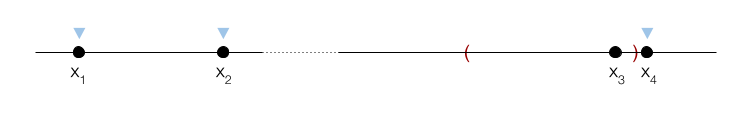
\includegraphics[width=12cm]{Images/imposibility1.png}
    \caption{$\x$}
    \label{fig:imp1}
\end{figure}

Let us remind the definition of the image set (Definition \ref{imageSet}). The image set of an agent $i$ is the set of facilities the agent can obtain by varying her reported location. Any interval in the complement of an image set $I_i(\x_{-i})$ is called a hole. By Lemma \ref{imageSetLemma} we have that the mechanism places a facility at the location in $I_i(\x_{-i})$ nearest to the location of agent $i$. Since agent $x_3$ is not allocated a facility in $\x$ there is a hole in the image set $I_3(\x_{-3})$ around $x_3$. Let $l$ and $r$ be the locations in $I_3(\x_{-3})$ nearest to $x_3$ on the left and on the right.(let the red lines represent the hole). Now consider the location profile $\y = (\x_{-3}, l+\epsilon)$. By Lemma \ref{imageSetLemma} the mechanisms should place a facility at $l$, since $l$ is the nearest location in the image set.


\begin{figure}[ht]
    \centering
    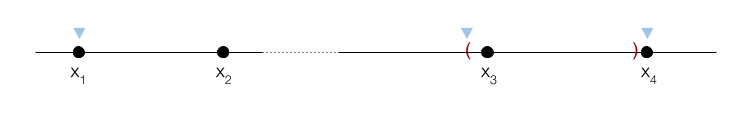
\includegraphics[width=12cm]{Images/imposibility2.png}
    \caption{$\y$}
    \label{fig:imp2}
\end{figure}

Now consider the location profile $\vec{z}=(\y_{-4},l)= (\x_{\{-3,4\}},\{l,l+\epsilon\})$. The mechanism is anonymous, which means we can rearrange the indices so that $x_1\le x_2 \le x_3\le x_4$. As a result, agents 3 and 4 switch indices in $\y$ and $\vec{z}$. We have that $M$ is strategyproof. Since in $\y$ and in $\vec{z}$ there is an agent at $l+\epsilon$ and in $\vec{z}$ an agent is moving closer to $l$, $M$ should keep a facility at $l$. By proposition \ref{left} we have that $x_4$ has a facility because $\x$ and $\vec{z}$ are well-separated instances and the nearby agents move to the right. But this way in $\vec{z}$ the nearby agents are allocated two facilities which makes the cost arbitrarily larger than the optimal.


%In $y$ and $z$ there is an agent at $l+\epsilon$. $M$ is strategyproof and since $M$ places a facility in $y$ at $l$ and in $z$ there is an agent at $l$, $M$ should keep a facility at $l$.
% In $\y$ and in $\vec{z}$ there is an agent at $l+\epsilon$ and in $\vec{z}$ an agent is moving closer to $l$. Since $M$ is strategyproof it should keep a facility at $l$


\begin{figure}[ht] 
    \centering
    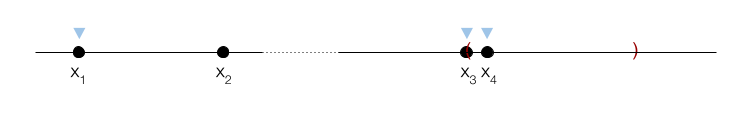
\includegraphics[width=12cm]{Images/imposibility3.png}
    \caption{$\vec{z}$}
    \label{fig:imp3}
\end{figure}



%---------------------------------------------------------------------------
% percentile mechanisms 
Even if we cannot have deterministic strategyproof mechanisms with a bounded approximation ration for the $k$-Facility Location games with $k\ge3$, there is a class of deterministic strategyproof mechanisms \cite{Sui2013}  for any $k\ge2$. A percentile mechanism splits the instance into $k$ parts, based on a predefined vector $\vec{p} \in (0,1)^k$, and allocates one facility at each part. One might think how can this class of mechanisms be practical if there is no guaranty for the outcome. However, in most ``real world" applications the designer has some knowledge of the preferences of the participating agents. This allows for empirical optimization of the vector $\vec{p}$. Let us formally define the percentile mechanisms.

\iffalse
\bigskip
Since we focus on anonymous mechanism we can assume without loss of generality that in an instance $\x = (x_1,...,x_n)$ all the agents' locations are in an ascending order ($x_1\le ... \le x_n$).  
\fi


\begin{definition}[$\vec{p}$-percentile mechanism]
The percentile mechanism is specified by a vector $\vec{p}=(p_1,...,p_k)$ where $0\le p_1\le...\le p_k \le 1$. The mechanism locates $j$th facility at the $p_j$th percentile of the reported locations. 
\[ c_j = x_{i_j}\; :\; i_j = \lfloor (n-1)\cdot p_j \rfloor +1 \]

\end{definition}

To better understand the mechanism let $\x = (x_1,...,x_9)$ be a location profile with $9$ agents. The $(0.25,0.75)$-percentile mechanism will place the first facility at $c_1=x_3$ since $\lfloor 8\cdot 0.25 \rfloor +1  = 3$ and the second facility at $c_2=x_7$ since $\lfloor 8\cdot 0.75 \rfloor +1 = 7$. 


\begin{figure}[ht]
    \centering
    
\includegraphics[width=12cm]{Images/percentile.png}
    \caption{Example of $(0.25,0.75)$-percentile mechanism for 9 agents}
    \label{fig:percentileExample}
\end{figure}

\begin{lemma}
The percentile mechanism is group strategyproof for any $\vec{p}$.
\end{lemma}

\begin{proof}
We are going to prove the lemma for $k=2$ but the proof is similar for $k\ge2$. Let $\vec{c}=(c_1,c_2)$ be the locations of the facilities when all the agents report their true preferences and $\vec{c}'=(c_1',c_2')$ be the locations after agents in a subset $S\subset N$ deviate from their true locations. Let $\Delta_1 = c_1-c_1'$ and $\Delta_2 = c_2'-c_2$. Now we need to show that at least one agent in $S$ does not benefit from the deviation. There are four cases to consider:
\begin{enumerate}[(i)]
    \item $\Delta_1\ge0$ and $\Delta_2>0$. That means that the first facility is moved to the left and the second to the right. In order for this to happen there is one agent that has an ideal location $x_i \in (c_1,c_2)$ who reported a location either to the left of $c_1$ or to the right of $c_2$. Otherwise the facilities could not move in such way. Now the cost of agent $i$ is:
    \begin{align*}
        cost(x_i,M(\xx)) &= min(d(x_i,c_1'),d(x_i,c_2'))\\
        &\ge min(d(x_i,c_1),d(x_i,c_2))\\
        &= cost(x_i,M(\x))
    \end{align*}
    \item $\Delta_1\ge0$ and $\Delta_2<0$. Now both facilities moved to the left. That means there is an agent $i$ with $x_i>c_2$, that reported a location to the left of $c_2$. Her cost is:
    \[ cost(x_i,M(\xx)) = x_i -c_2' \ge x_i-c_2 = cost(x_i,M(\x))\]
    \item $\Delta_1<0$ and $\Delta_2\ge0$. This case is completely symmetric to the previous case.
    \item $\Delta_1<0$ and $\Delta_2<0$. The first facility is moved to the right and the second to the left. As in the second case there is an agent to the right of $c_2$ that reported a location to the left. She cannot benefit from this deviation.
\end{enumerate}
Note that if $\Delta_1=0$ and $\Delta_2=0$ represents the case where neither facility moves and no agent benefits from the deviation. So without loss of generality we can assume that at least one of $\Delta_1$ or $\Delta_2$ is non-negative. 

\end{proof}
 
The main idea behind the proof is that the mechanism selects where to open a facility without ``looking" at the instance. Like in the example above in any instance (with $9$ agents) the $(0.25,0.75)$-percentile mechanism  will place the facilities at the $3$nd and $7$th agent respectively without looking at their actual locations. In order for an agent to change the outcome of the mechanism she would have to report a location $x'$ in a different part than her true preference. Like in the setting with one facility (and the median location) this deviation would move the facility further away making it a non profitable deviation. 


The \textsc{Two Extremes} mechanism mention above belongs in the class of percentile mechanism with a vector $\vec{p}=(0,1)$. It is also the only mechanism within the family of percentile mechanisms that has a bounded approximation ratio. For any $\vec{p}\neq (0,1)$ we can create an instance with arbitrarily small cost but since the mechanisms does not ``look" at the instance the solution will have arbitrarily large cost. Consider a location profile $\x=(0,\epsilon,1)$ where $\epsilon>0$ but arbitrarily close to $0$. The $(0,0.6)$- percentile mechanism will allocate the facilities to the first two agents. It is easy to see that the cost of the optimal solution is $\epsilon$ but the cost of the solution of the mechanism is $1-\epsilon$. Thus, the approximation ratio is unbounded.

~\\\textbf{Randomized mechanisms}

%{+Counter-example for proportional for 3 facilities+}
Again we may get better results if we consider randomized mechanism for $k$-Facility Location on the line. Unfortunately, a simple extensions of the proportional mechanism is not strategyproof even when $k=3$. The first two facilities are allocated like in the Proportional mechanism and the third is placed on a location of an agent with probability proportional to her minimal distance to the first two facilities. 

Consider this counter-example: there exist $n_0$ agents at $0$, $n_1$ agents at location $1$, $n_2$ agents at location $1+x$ and 1 agent at location $1+x+y$. Here $n_0$ is sufficiently large such that we can assume the first facility to be always located at $0$. In this configuration, let $y=100$, $x=10^{100}$, $n_1=50$ and $n_2=4$. An agent at location 1 may have the incentive to misreport to location 1+x. 

If we take a closer look at the instance, we can see that the distance between locations 0 and 1 is 1, and between locations $1+x$ and $1+x+y$ is $y$. By selecting $x=10^{100}$, the distance between locations 1 and $1+x$ is huge compared to the other two distances. By construction, the mechanism places the first facility at 0. Since the second facility is placed with a probability proportional to the distance to the first facility, the agent's deviation to $1+x$ increases the probability the second facility is placed at $1+x$. But that also means that the third facility  has an increased probability of being placed  at her true location, making that mechanism manipulable.




%{+Imposing mechanisms+}
Due to the negative results in the general setting new approaches were proposed. Imposing mechanisms was proposed by Nissim, Smorodinsky, and Tennenholtz \cite{Nissim2010}, namely mechanisms able to restrict how agents exploit their outcome. Fotakis and Tzamos \cite{Fotakis2013} showed that the winner-imposing version of the Proportional mechanism is strategyproof for the $k$-Facility Location game, and achieves an approximation ratio of at most $4k$. In this setting any agent that ``wins" a facility at her reported location must connect to it, even if there is a location closer to her ideal location. The mechanism runs in $k$ rounds and allocates one facility at each round. For each $\ell=1,...,k$ let $C_\ell$ denote the facility set after the $\ell$th round. 


\begin{definition}[Winner Imposing Proportional Mechanism]

Given a location profile $\vec{x}=(x_1,...x_n)$, the mechanism runs the following random process:
\begin{itemize}
    \item\textbf{Round 1:} Choose agent $i$ uniformly at random from $N$. The first facility is placed at $x_i$. Let $C_1=\{x_i\}$

    \item\textbf{Round $\ell$}, $\ell = 2,...,k$: Let $d_\ell = d(x_\ell,C_{\ell-1})$ be the distance from agent $\ell$ to the closest facility. Choose agent $\ell$ with probability $\frac{d_\ell}{\sum_{k\in N}d_k}$. The $\ell$th facility is placed at $x_\ell$, and agent $x_\ell$ connects to it. Let $C_\ell=C_{\ell-1}\cup \{x_\ell\}$

\end{itemize}
\end{definition}


%\subsubsection{Conclusion}

%conclution && different settings
%{+Equal cost?+}
%{?Verification?}

\section{Facility Location on general metrics}

In the section, we are going to present the most interesting results of the Facility Location games in more general metric spaces than the line. As we saw in the previous section, the problem becomes much more difficult as the number of facilities increases. In general metric areas, however, even the placement of one facility is not trivial.

\subsection{Tree Metrics}
The first metric space that we are going to focus on is the tree, because it has similar properties to the line. For the problem of locating one facility on a tree, we can obtain the same result as in the line. 

\begin{theorem}
The mechanism that selects the median location of the reported instance is strategyproof and optimal for the social cost objective.
\end{theorem}
\begin{proof}
Using the same arguments as in the line we can easily show that the median location is the optimal solution. The median on the tree is the location that when is viewed as the root all the subtrees have at most half of the nodes. Suppose the facility is placed at a location $x$ that is on subtree $T_1$. Then, the connection cost for all agents on $T_1$ (at most half) has decreased by $d(x,med(\vec{x}))$, but the connection cost for the rest of the agents (at least half) has increased by $d(x,med(\vec{x}))$. This makes the social cost of $x$ worst than the median location.

The median location is also strategyproof since the only way that an agent can change the median location is by reporting a location in a different subtree of the median. But this will only move the facility further away from her true location. 
\end{proof}

It gets a lot more complicated even if we consider $2$-Facility Location games on tree metric. For the next theorem we consider the star metric space. It consist of 3 half-lines $[0,\infty)$ with a common origin point $O$. We can see it as 3 long branches starting from $O$. So, we refer to this metric as $S_3$, and  to the branches as $b_1$,$b_2$ and $b_3$. A location $(x,b_l)$ in $S_3$ is determined by the distance $x\ge 0$ from the center and the corresponding branch. The distance between any two locations  $(x,b_l)$ and $(x',b_{l'})$ in $S3$ is $|x-x'|$, if $l=l'$ and $x+x'$ otherwise.

\begin{theorem}\cite{Fotakis2014}
Any deterministic strategy proof mechanism for 2-Facility Location game with $n\ge3$ agents in $S_3$ has an unbounded approximation ratio.
\end{theorem}

The proof again relies on well-separated instances with 3 agents. The idea is that even in those instances with an ``obvious" optimal solution, there is no deterministic and strategyproof way to determine where to place the facility that serves the two nearby agents.


\subsection{Circle}
We know that the tree is an acyclic graph, so the next natural question is what guarantees can we get when we have a circle. Schummer and Vohra \cite{Schummer2002} prove that any strategyproof and onto mechanism for locating one facility on a circle is dictatorial. 

%{?μπορεί και να μη χρειάζεται?}
The circle metric space $(S^1,d)$, where $S^1 \subset \mathbb{R}^2$ is a circle in the two dimensional Euclidean space and the distance function $d(x,y)$ for $x,y \in S^1$ is the length of the minor arc spanned by $x$ and $y$.  


The approximation ratio of any dictatorial mechanism is $n-1$. This can be verified by a simple example. Suppose $n-1$ agents are located at $x$ and one agent is located at $y$. The obvious optimal solution is to place the facility at $x$ with social cost equal to $d(x,y)$. If the dictator is located at $y$ then the social cost of that solution is equal to $(n-1)d(x,y)$  


Once again, we can use randomization to get a better approximation ratio. By selecting uniformly at random any location we can achieve constant approximation ratio.

\begin{definition}[Random Dictator]
The mechanism that selects a location uniformly at random from the reported locations is strategyproof and has an approximation ratio of $2-\frac{2}{n}$.
\end{definition}

\begin{proof}
The mechanism is strategyproof because an agent that deviates if selected loses since the location is further away from her ideal location and, if not selected, cannot change the outcome of the mechanism.

For the approximation ratio, let $y$ be the optimal solution. Since the mechanism selects a location uniformly at random the expected social cost is:
\begin{align*}
    cost(\x,M(\x)) &= \frac{1}{n} \sum_{i\in N}\sum_{j\ne i} d(x_i,x_j)  \\
    &=\frac{1}{n} \sum_{i\in N}\sum_{j\ne i} d(x_i,y)+d(y,x_j)\\
    &=\frac{1}{n} \sum_{i\in N} \Big( (n-1)d(x_i,y) + SC^*-d(x_i,y) \Big)\\
    &= \frac{1}{n}\sum_{i\in N} \Big( (n-2)d(x_i,y) + SC^* \Big)\\
    &=SC^* + \frac{n-2}{n}SC^*
\end{align*}
\end{proof}

There is also a mechanism for 2-Facilities in a circle. Since the mechanism for one facility in the circle is dictatorial, we cannot expect that to change for 2 facilities. The mechanism works as follows: it places the first facility at the location of the dictator, then it cuts the circle in half and allocates the second facility based on the maximum distance in each semi-circle to the first facility.


\begin{definition}[Circle mechanism for 2 Facilities]
Given a location profile $\vec{x}=(x_1,...x_n)$ the first facility is allocated at $x_1$, the location of the first agent. Let $\hat{x}_1$ denote the antipodal of $x_1$. There are two semi-circles formed with $x_1$ and $\hat{x}_1$ as endpoints, the left circle $\mathcal{L}$ and the right circle $\mathcal{R}$. Let $\mathcal{A}$ and $\mathcal{B}$ be the set of agents on $\mathcal{L}$ and $\mathcal{R}$ respectively. We assume agents at location $x_1$ and $\hat{x}_1$  appear only in $\mathcal{A}$, and thus $\mathcal{A}\cap \mathcal{B}= \emptyset$. Define $d_A = max_{i \in \mathcal{A}} d(x_1,x_i)$ and $d_B = max_{i \in \mathcal{B}} d(x_1,x_i)$. If $\mathcal{B}$ is empty then $d_B = 0$. The second facility is allocated as follows:
\begin{itemize}
    \item If $d_A < d_B$ facility $c_2$ is placed on $\mathcal{R}$ with distance $min\{max\{ d_B, 2d_A\},1/2 \}$ to $c_1$ 
    \item If $d_A \ge d_B$ facility $c_2$ is placed on $\mathcal{L}$ with distance $min\{max\{ d_A, 2d_B\},1/2 \}$ to $c_1$
\end{itemize}
\end{definition}



\begin{theorem}\cite{Lu2010}
The circle mechanism for the $2$-Facility Location game is strategyproof and has an approximation ratio of at most $n-1$
\end{theorem}

There is a simple instance for which the circle mechanism has an approximation ration equal to $n-1$. Consider the location profile $\x=(x_1,...,x_n)$, where $d(x_1,x_2)=d(x_1,x_3)=0.1$ and $x_3,...x_n$. But $x_2$ and $x_3$ are in different sides of $x_1$. The optimal solution is to place one facility at $x_1$ (or $x_2$) and the second facility at $x_3$. The cost of the optimal solution is 0.1. But the circle mechanism will place one facility at $x_1$ and the second facility at the left semi-circle at a distance 0.2 to the first. The cost is $(n-1)0.1$

\subsection{Euclidean Space}
%coordinate wise median location 

For a set of points in a two dimensional Euclidean space the geometric median is the point that minimizes the sum of the distances to the data points. The distance function is the $L_2$-Norm. Formally given a set of points $x_1,...,x_n\in R^m$ the geometric median is:
\[ med =  \underset{y\in\mathbb{R}^2}{\mathrm{argmin}}  \bigg\{ \sum_{i=1}^n d(x_i,y) \bigg\} \]


However, the geometric median can only be approximated. 


\begin{definition}
In the Euclidean metric space with $X = \mathbb{R}^m$, a mechanism f is called a generalized coordinate-wise median voting scheme with k constant points if there exists a coordinate system and points $a_1,...,a_k \in (\mathbb{R}\cup \{-\infty,\infty\})^m$ so that for every profile $\x \in \mathbb{R}^m$ and every $j=1,2,...,m$:

\[M^j(\x) \coloneqq \text{med}(x_1^j,x_2^j,...,x_n^j,a_1^j,...,a_k^j)\]

Where ``med" denotes the median of the subsequent real numbers, and all coordinates are expressed with respect to the given coordinate system. 

\end{definition}
 

\begin{lemma}\cite{Peters1992}
In the Euclidean metric space with $X=\mathbb{R}^2$ and an odd number of agents, a mechanism $M$ is Pareto optimal, anonymous and strategyproof if, and only if, it is a coordinate-wise median scheme with 0 constant points.
\end{lemma}
The coordinate-wise median is strategyproof because it handles each coordinate separately. Using the same ideas as in the median on the line, the only way to change the median location is by reporting a location on the other side. But this will move the median further away.   



\begin{lemma} \cite{Meir2019}
For $X=\mathbb{R}^m$ and  the social cost objective, the coordinate-wise median mechanism has an approximation ratio of at most $\sqrt{m}$ for any number of agents $n$.
\end{lemma}



%\subsubsection{Conclusion}










\section{Conclusion}

In this chapter, we look at various settings for the $k$-Facility Location games. However, the goal was the same: the design of a mechanism with desirable proprieties such as strategyproofness, Pareto optimality, anonymity, and a bounded approximation ratio. Unfortunately, in most cases, this was infeasible. Since strategyproofness is a property we always want to have, we need to sacrifice one of the other two properties. We can have strategyproofness and a bounded approximation ratio on the circle metric space, but not anonymity since the mechanisms admit a dictator. On the other hand, in the case of the percentile mechanism, we have strategyproofness and anonymity but not a bounded approximation ratio. The trade-off between strategyproofness and approximability is the most interesting because it shows that those properties are incompatible. Intuitively, to achieve a bounded approximation ratio in the multi-facility setting, we need to place one facility in each optimal cluster; otherwise, we can construct an instance with an unbounded approximation ratio. But, as we saw for 3-Facility Location games with 4 agents, there is no deterministic strategyproof way to identify the optimal clusters and place the facilities even in well-separated instances.